
\documentclass[titlepage, a4paper]{article}
\usepackage[swedish]{babel}
\usepackage[utf8]{inputenc}
\usepackage{color}

% Sidformat
\usepackage{a4wide}

% Fixa Appendix-titlar
\usepackage[titletoc,title]{appendix}

% Bättre bildtexter
\usepackage[margin=10pt,font=small,labelfont=bf,labelsep=endash]{caption}

% Enkelt kommando som låter mig attgöra-markera text
\newcommand{\todo}[1] {\textbf{\textcolor{red}{#1}}}

%% Headers och Footers
\usepackage{fancyhdr}
\pagestyle{fancy}
\lhead{}
\rhead{\today}
\lfoot{\LIPSkursnamn \\ \LIPSdokumenttyp}
\cfoot{\thepage}
\rfoot{\LIPSprojektgrupp \\ \LIPSprojektnamn}

%% Titelsida
\newcommand{\LIPSTitelsida}{%
{\ }\vspace{45mm}
\begin{center}
  \textbf{\Huge \LIPSdokument}
\end{center}
\begin{center}
  {\Large Redaktör: \LIPSredaktor}
\end{center}
\begin{center}
  {\Large \textbf{Version \LIPSversion}}
\end{center}
\vfill
\begin{center}
  {\large Status}\\[1.5ex]
  \begin{tabular}{|*{3}{p{40mm}|}}
    \hline
    Granskad & \LIPSgranskare & \LIPSgranskatdatum \\
    \hline
    Godkänd & \LIPSgodkannare & \LIPSgodkantdatum \\
    \hline
  \end{tabular}
\end{center}
\newpage
}


% Projektidentitet
\newenvironment{LIPSprojektidentitet}{%
{\ }\vspace{45mm}
\begin{center}
  {\Large PROJEKTIDENTITET}\\[0.5ex]
  {\small
  \LIPSartaltermin, \LIPSprojektgrupp\\
  Linköpings Tekniska Högskola, MAI
  }
\end{center}
\begin{center}
  {\normalsize Gruppdeltagare}\\
  \begin{tabular}{|l|l|p{25mm}|l|}
    \hline
    \textbf{Namn} & \textbf{Ansvar} & \textbf{Telefon} & \textbf{E-post} \\
    \hline
}%
{%
    \hline
  \end{tabular}
\end{center}
\begin{center}
  {\small
    \textbf{E-postlista för hela gruppen}: \LIPSgruppadress\\
    \textbf{Hemsida}: \LIPSgrupphemsida\\[1ex]
    \textbf{Kund}: \LIPSkund\\
    \textbf{Kontaktperson hos kund}: \LIPSkundkontakt\\
    \textbf{Kursansvarig}: \LIPSkursansvarig\\
    \textbf{Handledare}: \LIPShandledare\\
  }
\end{center}
\newpage
}
\newcommand{\LIPSgruppmedlem}[4]{\hline {#1} & {#2} & {#3} & {#4} \\}

%% Dokumenthistorik
\newenvironment{LIPSdokumenthistorik}{%
\begin{center}
  Dokumenthistorik\\[1ex]
  %\begin{small}
    \begin{tabular}{|l|l|p{60mm}|l|l|}
      \hline
      \textbf{Version} & \textbf{Datum} & \textbf{Utförda förändringar} & \textbf{Utförda av} & \textbf{Granskad} \\
      }%
    {%
			\hline
    \end{tabular}
  %\end{small}
\end{center}
}

\newcommand{\LIPSversionsinfo}[5]{\hline {#1} & {#2} & {#3} & {#4} & {#5} \\}

% Kravlistor
\newenvironment{LIPSkravlista}{
	\center
		\tabularx{\textwidth}{| p{1.2cm} | p{1.9cm} | X | c |}
			\hline
			\textbf{Krav} & \textbf{Förändring} & \textbf{Beskrivning} & \textbf{Prioritet} \\\hline
}
{
		\endtabularx
	\endcenter
}

\newcounter{LIPSkravnummer}
\addtocounter{LIPSkravnummer}{1}
\newcommand{\LIPSkrav}[4][Krav \arabic{LIPSkravnummer}]{{#1} & {#2} & {#3} & {#4} \stepcounter{LIPSkravnummer}\\\hline}	% Importera generella layout-strukturer

% Information nödvändig för generella layout-strukturer
\newcommand{\LIPSredaktor}{Daniel Wassing}
\newcommand{\LIPSversion}{0.1}
\newcommand{\LIPSdokument}{Användarhandledning}
\newcommand{\LIPSdokumenttyp}{Användarhandledning}
\newcommand{\LIPSgranskatdatum}{}
\newcommand{\LIPSgranskare}{}
\newcommand{\LIPSgodkannare}{}
\newcommand{\LIPSgodkantdatum}{}
\newcommand{\LIPSkursnamn}{TSEA29}
\newcommand{\LIPSprojektnamn}{Lagerrobot}
\newcommand{\LIPSprojektgrupp}{Grupp 2}
%\newcommand{\LIPSgruppadress}{}
\newcommand{\LIPSartaltermin}{HT1, 2014}
\newcommand{\LIPSgrupphemsida}{http://github.com/ultralaserdeluxe/gloria}
\newcommand{\LIPSkund}{Tomas Svensson}
\newcommand{\LIPSkundkontakt}{Tomas Svensson}
\newcommand{\LIPSkursansvarig}{Tomas Svensson}
\newcommand{\LIPShandledare}{Peter Johansson}

% Dokument-specifika paket
\usepackage{tabularx}
\usepackage{subcaption}
\usepackage{tikz}
\usepackage{mathtools}
\usetikzlibrary{shapes, arrows}

\pagenumbering{roman}

\begin{document}

\LIPSTitelsida

\begin{LIPSprojektidentitet}
\LIPSgruppmedlem{Pål Kastman}{Projektledare}{0703896295}{palka285@student.liu.se}
\LIPSgruppmedlem{Hannes Snögren}{Dokumentansvarig}{0706265064}{hansn314@student.liu.se}
\LIPSgruppmedlem{Alexander Yngve}{Hårdvaruansvarig}{0762749762}{aleyn573@student.liu.se}
\LIPSgruppmedlem{Martin Söderén}{Mjukvaruansvarig}{0708163241}{marso329@student.liu.se}
\LIPSgruppmedlem{Daniel Wassing}{Leveransansvarig}{0767741110}{danwa223@student.liu.se}
\LIPSgruppmedlem{Dennis Ljung}{Testansvarig}{0708568148}{denlj069@student.liu.se}
\end{LIPSprojektidentitet}

\newpage
\tableofcontents	%Innehållsförteckning
%\listoffigures
%\listoftables

\newpage

\begin{LIPSdokumenthistorik}
\LIPSversionsinfo{0.1}{2014-12-15}{Första utkast}{danwa223}{}
\LIPSversionsinfo{0.2}{2014-12-16}{Första inlämning}{danwa223}{}
\end{LIPSdokumenthistorik}

\newpage
\pagenumbering{arabic}	%Påbörja sidnumrering

% Inledning, översikt osv
\section{Inledning}

Det här dokumentet är en sammanfattad guide till hur man kan använda lagerroboten Gloria, skapad av grupp 2 för TSEA29 HT2014.
\newline
\newline
Syftet är att man med hjälp av denna användarhandledning enkelt ska kunna sätta upp en miljö för att ansluta, konfigurera och styra gloria.
\section{Användning av systemet}

\subsection{Ansluta till Huvudenheten}
\todo{Direkt från tekdok. Kan behöva redigeras för att passa in}
För att ansluta en ny dator med Linux till huvudenhetens PAN behövs följande göras:
\todo{får uppdatera detta, osäker om detta stämmer}
\begin{enumerate}
	\item ha tillgång till en terminal på huvudenheten, den enklaste är att ansluta en skärm och tangentbord till den.\newline Lösenordet är :"temppwd"
	\item kör "sudo bluez-simple-agent hci0 xx:xx:xx:xx:xx:xx" där du byter ut kryssen mot din blåtandenhets mac-adress
	\item paira huvudenheten med din pc från din pc
	\item  kör "sudo bluez-test-device trusted xx:xx:xx:xx:xx:xx yes" på huvudenheten
	\item du kan nu ta bort pairing från din pc
	\item kör "sudo pand -n -c 00:19:0E:0F:F0:6F	" på din pc
	\item kör "sudo ifconfig bnep0 192.168.99.2 up " på din pc
\end{enumerate}
Nu borde du kunna pinga och ssh in på ubuntu@192.168.99.1 vilket är huvudenhetens statiska ip-adress. I framtiden behövs bara de två sista stegen genomföras.

\section{Styrning av robot}
\subsection{Start av Mjukvara}
\begin{enumerate}
	\item Om anslutning har etablerats till Gloria så behöver man hitta filen mainThread.py som ligger i home directory, dvs där man hamnar när man väl har ssh:at in (se Användning av Systemet).
	\item Kommandot för att starta systemet i Gloria är bara en rad: python mainThread.py
	När detta kommandot körs så sätter systemet igång och Gloria lägger sig i vänteläge.
	\item Efter att mainThread.py har startats på Gloria så startar man upp en ny terminal lokalt på datorn som Gloria ska styras ifrån och hittar Gui.py. Sedan kör man kommandot: python Gui.py
	\item Anslut två joysticks via USB (till pc). Klargör vilken som styr motor och vilken som styr arm.
\end{enumerate}
\subsection{Användning av Mjukvara}
\begin{enumerate}
	\item Styrning av Gloria sker som följer: 
	\begin{itemize}
		\item Väl inne i Gui.py, tryck på \textbf{connect arm joystick} för att ansluta joysticken som styr armen.
		\item Samma procedur gäller för joysticken som styr motorn.
		\item Ange Glorias statiska IP-adress (192.168.99.1) i connect-fältet och tryck på \textbf{connect}.
		\item Motor: Joystick 1 låter användaren köra i alla riktningar. Framåt-tilt får Gloria att accelerera framåt, bakåt-tilt ger samma effekt bakåt. Vänster orsakar en vänstersväng (vänster hjulpar kör långsammare än höger) och höger fungerar på samma sätt.
		\item Arm: Armen (Gripklon) styrs i ett 3D-rum utifrån hur man rör Joystick 2 där gripklon är koordinaten i planet. Rörelserna beräknas automatiskt, så dessa behöver användaren inte ta hänsyn till. 
		\item Gripklo framåt/bakåt/vänster/höger: Tilta Joysticken i önskad rikting.
		\item Höj/Sänk Gripklon: %todo
		\item Rotera vristen: Vrid Joysticken åt vänster/höger
		\item Gripklo (släpp, grepp): Höger pedal på baksida av Joysticken regleras från 0 till 1, där 0 innebär att gripklon är helt öppen och 1 innebär att den är stängd.
		
	\end{itemize}
	\item Knapparna i nedre vänstra hörnet på GUI gör följande:
	\begin{itemize}
		\item start: Startar Glorias mainloop, behöver göras innan några andra kommandon kan accepteras.
		\item calibrate tape: Kalibrerar sensorvärdet för tejp.
		\item calibrate floor: Kalibrerar sensorvärdet för golv.
		\item got package: Signalerar till Gloria att man är klar med att plocka upp ett packet med Joysticken.
		\item auto motor: Sätter motorerna i autonomt läge, vilket får Gloria att köra av sig själv givet sensordata.
		\item auto arm: Sätter armen i autonomt läge.
	\end{itemize}
	\begin{figure}[h]
	\center
	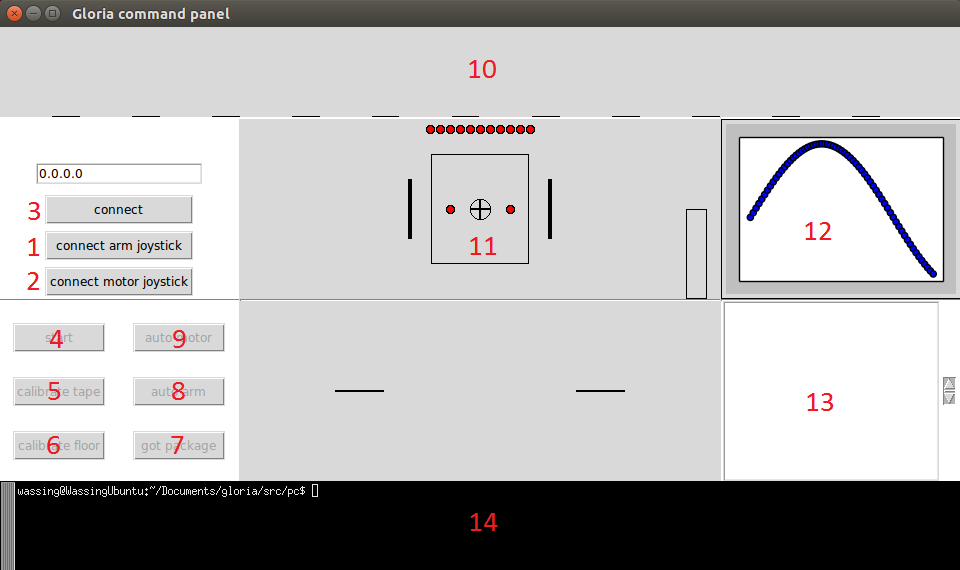
\includegraphics[scale=0.6]{Gui.png}
	\endcenter
	\caption{Gui. Överst visas sensordata, i mitten visas gloria, till vänster alla relevanta knappar, till höger visas reglerfel samt errorcodes och nederst visas en terminal.}
	\end{figure}
\end{enumerate}
\clearpage
\newpage
\begin{appendices}
% Bilagor
\section{Banregler} \label{banregler}

Banan är uppmärkt med en tejp som är mellan 14-18mm tjock. Banan får korsa sin egen väg, med restriktionen att det skall ske rätvinkligt. Där banan korsar sin egen väg skall den vara rak i minst 30cm från korsningen. Avbrott i banan får förekomma, under förutsättning att det sker på en raksträcka och avbrottet inte är längre än 10 cm. Banans svängradie får ej understiga 25cm. \\
Det finns minst ett paket vid banan. \\
Upplockningsstationer är markerade med en vinkelrät tejp åt den sida på vilken stationen finnes. Antalet upplockningsstationer är större än antalet paket. \\
En slutmarkering är inte nödvändig för banans giltighet. Finns det ett stop markeras det av två parallella tejpbitar vinkelräta mot banan samt en vinkelrät tejpbit, placerad mellan de två markeringarna som leder till robotens förvaringsutrymme.


\end{appendices}


\end{document}
